% !TEX root = ../../math6370.tex
\section{Geometry of Numbers}
\subsection{Minkowski Theory}

\begin{dfn}[Euclidean Space]
A Euclidean space is a finite dimensional real inner product space $\langle \cdot\,,\,\cdot\rangle: V \times V \to \R$.
\end{dfn}

\begin{ex}
The pair $(\R^n, \cdot)$, where $\cdot$ is the usual dot product, is a Euclidean space. \xqed
\end{ex}

Recall that if $H$ is an additive subgroup of a vector space $V$ that $H$ is discrete if and only if $H$ is a free $\Z$-module generated by linearly independent vectors over $\R$. 

\begin{ex}
Both $\Z \subseteq \C$ and $\Z^2 \subseteq \R^2$ are discrete. 
	\begin{figure}[h!]
	\centering
	\begin{tikzpicture}
	\clip (-3.3,-3.3) rectangle (3.3cm,3.3cm); % Clips the picture...
    		\coordinate (Origin)   at (0,0);
    		\coordinate (XAxisMin) at (-3.3,0);
    		\coordinate (XAxisMax) at (3.3,0);
    		\coordinate (YAxisMin) at (0,-3.3);
    		\coordinate (YAxisMax) at (0,3.3);
    		\draw [thin,-latex] (XAxisMin) -- (XAxisMax);% Draw x axis
    		\draw [thin,-latex] (YAxisMin) -- (YAxisMax);% Draw y axis	
		
		\foreach \Point in {(-3,0),(-2,0),(-1,0),(0,0),(1,0),(2,0),(3,0)}{\node at \Point{\textbullet};}
			
    		\draw[style=help lines,dashed] (-4,-4) grid[step=1cm] (4,4);
	\end{tikzpicture} \hspace{1cm}
	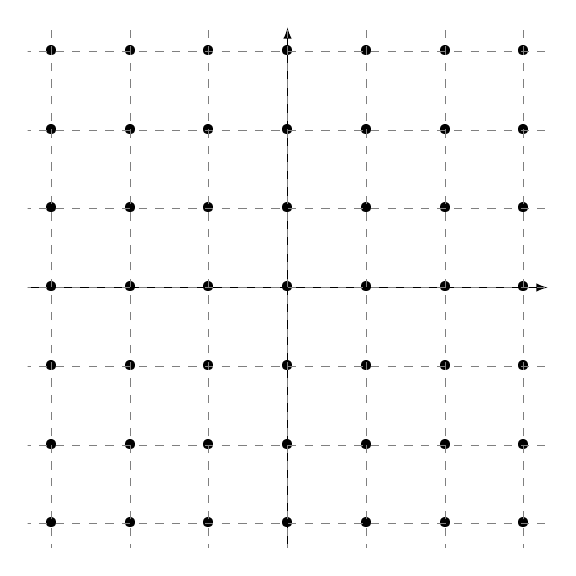
\begin{tikzpicture}
	\clip (-3.3,-3.3) rectangle (3.3cm,3.3cm); % Clips the picture...
    		\coordinate (Origin)   at (0,0);
    		\coordinate (XAxisMin) at (-3.3,0);
    		\coordinate (XAxisMax) at (3.3,0);
    		\coordinate (YAxisMin) at (0,-3.3);
    		\coordinate (YAxisMax) at (0,3.3);
    		\draw [thin,-latex] (XAxisMin) -- (XAxisMax);% Draw x axis
    		\draw [thin,-latex] (YAxisMin) -- (YAxisMax);% Draw y axis	
		
		\foreach \Point in {(-3,-3),(-2,-3),(-1,-3),(0,-3),(1,-3),(2,-3),(3,-3)}{\node at \Point{\textbullet};}
		\foreach \Point in {(-3,-2),(-2,-2),(-1,-2),(0,-2),(1,-2),(2,-2),(3,-2)}{\node at \Point{\textbullet};}
		\foreach \Point in {(-3,-1),(-2,-1),(-1,-1),(0,-1),(1,-1),(2,-1),(3,-1)}{\node at \Point{\textbullet};}
		\foreach \Point in {(-3,0),(-2,0),(-1,0),(0,0),(1,0),(2,0),(3,0)}{\node at \Point{\textbullet};}
		\foreach \Point in {(-3,1),(-2,1),(-1,1),(0,1),(1,1),(2,1),(3,1)}{\node at \Point{\textbullet};}
		\foreach \Point in {(-3,2),(-2,2),(-1,2),(0,2),(1,2),(2,2),(3,2)}{\node at \Point{\textbullet};}
		\foreach \Point in {(-3,3),(-2,3),(-1,3),(0,3),(1,3),(2,3),(3,3)}{\node at \Point{\textbullet};}
			
    		\draw[style=help lines,dashed] (-4,-4) grid[step=1cm] (4,4);
	\end{tikzpicture}
	\caption{The lattice for $\Z \subseteq \C$ (left) and $\Z^2 \subseteq \R^2$ (right). \label{fig:discretelattice}}
	\end{figure} 
\xqed
\end{ex}


\begin{dfn}[Lattice]
A subgroup $\Lambda \subseteq V$ is a lattice if it is discrete and spans $V$ over $\R$; that is, 
	\[
	\Lambda= \Z v_1 \oplus \Z v_2 \oplus \cdots \Z v_n,
	\]
where $v_1,\ldots,v_n$ a basis for $V$ over $\R$. 
\end{dfn}

\begin{rem}
What we here refer to as a lattice is sometimes referred to as a complete or full lattice. 
\end{rem}

On $V$, we have a volume measure on $V$ --- the Haar measure $\mu$: $\mu(\{x_1e_1+\cdots+x_ne_n \colon 0 \leq x_i<1\})=1$, where $e_1,\ldots,e_n$ is an orthonormal basis.

\begin{dfn}[Fundamental Domain]
Let $\Lambda \subseteq V$ be a lattice with $\Lambda= \Z v_1 \oplus \Z v_2 \oplus \cdots \Z v_n$. A fundamental domain for $\Lambda$ is
	\[
	\cF:=\{ x_1v_1 + \cdots + x_nv_n \colon 0 \leq x_i<1\}.
	\]
\end{dfn}

\begin{ex}
A fundamental domain for the lattice in $\R^2$ generated by the vectors $\langle1,1\rangle$ and $\langle\sqrt{2},-\sqrt{2}\rangle$ is the region shaded in the Figure~\ref{fig:fundex} below.
	\begin{figure}[h!]
	\centering
	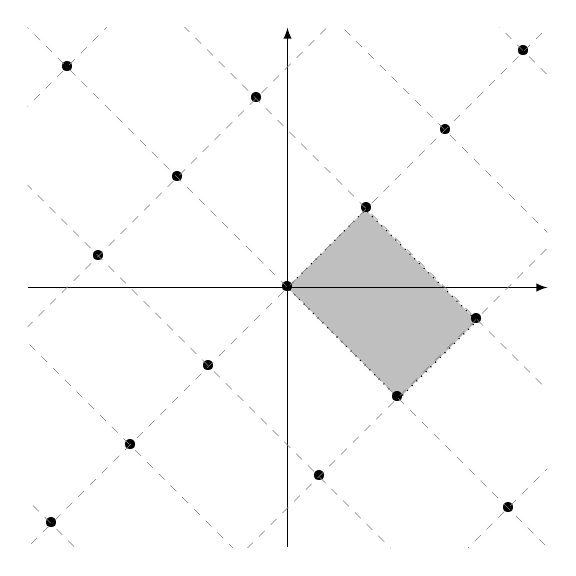
\begin{tikzpicture}
	\clip (-3.3,-3.3) rectangle (3.3cm,3.3cm); % Clips the picture...
	
		\draw[dotted,rotate around={-45:(0,0)},fill=lightgray] (0,0) rectangle (2,1.4);		
		
    		\coordinate (Origin)   at (0,0);
    		\coordinate (XAxisMin) at (-3.3,0);
    		\coordinate (XAxisMax) at (3.3,0);
    		\coordinate (YAxisMin) at (0,-3.3);
    		\coordinate (YAxisMax) at (0,3.3);
    		\draw [thin,-latex] (XAxisMin) -- (XAxisMax);% Draw x axis
    		\draw [thin,-latex] (YAxisMin) -- (YAxisMax);% Draw y axis	
		
		\foreach \Point in {
		(-7.2, 1.2), (-5.8, -0.2), (-4.4, -1.6), (-3., -3.), (-1.6, -4.4),(-0.2, -5.8), (1.2, -7.2), (-6.2, 2.2), (-4.8, 0.8), (-3.4, -0.6),(-2., -2.), (-0.6, -3.4), (0.8, -4.8), (2.2, -6.2), (-5.2, 3.2),(-3.8, 1.8), (-2.4, 0.4), (-1., -1.), (0.4, -2.4), (1.8, -3.8), (3.2,-5.2), (-4.2, 4.2), (-2.8, 2.8), (-1.4, 1.4), (0., 0.), (1.4, -1.4),(2.8, -2.8), (4.2, -4.2), (-3.2, 5.2), (-1.8, 3.8), (-0.4, 2.4), (1.,1.), (2.4, -0.4), (3.8, -1.8), (5.2, -3.2), (-2.2, 6.2), (-0.8, 4.8),(0.6, 3.4), (2., 2.), (3.4, 0.6), (4.8, -0.8), (6.2, -2.2), (-1.2,7.2), (0.2, 5.8), (1.6, 4.4), (3., 3.), (4.4, 1.6), (5.8, 0.2), (7.2,-1.2)
		}{\node at \Point{\textbullet};}

		\pgftransformcm{1}{1}{1.4}{-1.4}{\pgfpoint{0cm}{0cm}}			
    		\draw[style=help lines,dashed] (-4,-4) grid[step=1cm] (4,4);
	\end{tikzpicture}
	\caption{The fundamental domain of $\Z[\sqrt{2}]$ generated by $\langle1,1\rangle$ and $\langle\sqrt{2},-\sqrt{2}\rangle$. \label{fig:fundex}}
	\end{figure}
\end{ex}

Note that we have
	\[
	V= \bigcup_{\lambda \in \Lambda} (\lambda + \cF).
	\]
The Haar measure on $V$ assigns volume 1 to the fundamental domain and we say that
	\[
	\vol(\cF):= \mu(\cF).
	\]

\begin{dfn}[Covolume]
The covolume of $\Lambda= \Z v_1 \oplus \cdots \oplus \Z v_n$ is $\covol(\Lambda):= \vol(\cF)=\mu(\cF)$.
\end{dfn}

The covolume of $\Lambda$ is independent of the $v_i$. If $e_1,\ldots,e_n$ is an orthonormal basis for $V$. Write
	\[
	v_i= \sum_{j=1}^n A_{ij} e_j
	\]
for a unique $A \in \GL_n(\R)$. Then $\vol(\cF)=|\det A|$ (the absolute value removes sign issues that could arise). The matrix $B:=B_{ij}= (\langle v_i,v_n \rangle)_{i,j}$ satisfies $B=AA^T$, and $\covol(\Lambda)=\vol(\cF)=|\det((\langle v_i,v_j \rangle)_{i,j})|^{1/2}=\sqrt{|\det B|}$. 


\begin{rem}
The quotient map $V \to V/\Lambda$ gives a way of relating volume and covolume. The space $V/\Lambda$ is compact and has Haar measure $\overline{\mu}$ --- the one induced from $\mu$ on $V$.
	\[
	\vol(V/\Lambda)= \overline{\mu}(V/\Lambda)=\mu(\cF)=\covol(\Lambda)
	\]
\end{rem}



\subsection{Lattices from $\O_K$}

Let $K$ be a number field of degree $n$. Let $\sigma: K \hookrightarrow \C$ be a complex embedding of $K$ to $\C$. Recall that we have a map
	\[
	K_\R:= \{ (a_\sigma) \in \prod_\sigma \C \colon \overline{a_\sigma}= a_{\overline{\sigma}} \text{ for all }\sigma: K \hookrightarrow \C\},
	\]
where $\sigma$ runs over all complex embeddings $\sigma: K \hookrightarrow \C$ and $\overline{\sigma}$ is the complex conjugate embedding of $\sigma$ given by $\text{conj} \circ \sigma$ with $\text{conj}$ being complex conjugation. Now $K_\R$ is a real vector space of dimension $n$. There is a map
	\[
	\begin{tikzcd}
	K \arrow[hook]{r} & K_\R \\[-3ex]
	\alpha \arrow[mapsto]{r} & \big(\sigma(\alpha)\big)_{\sigma}
	\end{tikzcd}
	\]
that induces an isomorphism of $\R$-algebras $K \otimes_\Q \R \stackrel{\sim}{\to} K_\R$. We have seen that $\Lambda:= i(\O_K)$ is a lattice in $K_\R$: $\O_K \cong \Z^n \subseteq K \cong \Q^n$ as additive abelian groups. 
	\[
	\begin{tikzcd}
	\O_K \arrow[draw=none]{r}[sloped,auto=false]{\cong} \arrow[draw=none]{d}[sloped,auto=false]{\subseteq}  & \Z^n \arrow[draw=none]{d}[sloped,auto=false]{\subseteq} \\
	K \arrow[draw=none]{r}[sloped,auto=false]{\cong} & \Q^n
	\end{tikzcd}
	\]
For a nonzero ideal $I \subseteq \O_K$, $i(I)$ is a lattice in $K_\R$. We want an inner product on $K_\R$. Recall that we had a symmetric, positive definite, bilinear pairing
	\[
	\begin{tikzcd}
	K \times K \arrow{r} \arrow{r} & \Q \\[-3ex]
	(\alpha,\beta) \arrow[mapsto]{r} & \Tr{K/\Q}(\alpha \beta)
	\end{tikzcd}
	\]
where
	\[
	\Tr{K/\Q}(\alpha \beta) = \sum_{\sigma: K \hookrightarrow \C} \sigma(\alpha)\sigma(\beta).
	\]
Define a pairing $\langle \;,\; \rangle: K_\R \times K_\R \to \R$ by
	\[
	\begin{tikzcd}
	\langle \;,\; \rangle: K_\R \times K_\R \arrow[hook]{r} & \R \\[-3ex]
	\big( (a_\sigma)_\sigma, (b_\sigma)_\sigma \big) \arrow[mapsto]{r} & \displaystyle\sum_\sigma a_\sigma b_\sigma
	\end{tikzcd}
	\]
The image of this pairing is indeed in $\R$ as
	\[
	\overline{\sum_\sigma a_\sigma b_\sigma} = \sum_\sigma \overline{a_\sigma} \; \overline{b_\sigma} = \sum_\sigma a_{\overline{\sigma}} \;b_{\overline{\sigma}} = \sum_\sigma a_\sigma b_\sigma.
	\]
The pairing is clearly bilinear and symmetric. It only remains to show that the pairing is positive definite but this is clear as $\langle i(\alpha), i(\beta)\rangle = \Tr{K/\Q}(\alpha \beta)$ for $\alpha,\beta \in K$. 


Now let $r$ be the number of embeddings $\sigma: K \hookrightarrow \R$ (the real embeddings) and let $s$ be the number of complex conjugate pairs of embeddings $\sigma: K \hookrightarrow \C$ with $\sigma(K) \not\subseteq \R$ (the complex embeddings). Since $K$ has degree $n$, $n=r+2s$. Order the embeddings as follows: \\
	\begin{itemize}
	\item $\sigma_1,\ldots,\sigma_r$ the real embeddings of $K$ \\
	\item $\sigma_{r+1},\ldots,\sigma_{r+s}, \overline{\sigma_{r+1}}, \ldots, \overline{\sigma_{r+s}}$ the complex embeddings of $K$.
	\end{itemize}
Then we have $K_\R \cong \R^r \times \R^{2s} \cong \R^n$ using the isomorphism
	\[
	(a_\sigma)_\sigma \mapsto \bigg(a_{\sigma_1}, \ldots, a_{\sigma_r}, \ream(a_{\sigma_{r+s}}), \ldots, \ream(a_{\sigma_{r+s}}), \imag(a_{\sigma_{r+1}}), \ldots, \imag(a_{\sigma_{r+s}}) \bigg).
	\]
We have an inner product on the left hand side given by 
	\[
	\begin{split}
	\langle (a_\sigma), (b_\sigma) \rangle&= \sum_\sigma a_\sigma b_\sigma \\
	&= \sum_{i=1}^r a_{\sigma_i} b_{\sigma_i} + \sum_{i=r+1}^{r+s} \left( a_{\sigma_i} b_{\sigma_i} + \overline{a_{\sigma_i}} \; \overline{b_{\sigma_i}} \right) \\
	&= \sum_{i=1}^r a_{\sigma_i} b_{\sigma_i} + \sum_{i=r+1}^{r+s} \bigg(2 \ream(a_{\sigma_i}) \ream(b_{\sigma_i}) + 2 \imag(a_{\sigma_i}) \imag(b_{\sigma_i}) \bigg)
	\end{split}
	\]
This forces us into the following choice for an inner product on $\R^n$:
	\[
	\begin{tikzcd}
	\R^n \times \R^n \arrow{r} & \R \\[-3ex]
	\langle x,y \rangle \arrow[mapsto]{r} & \displaystyle \sum_{i=1}^r x_iy_i + 2 \sum_{i=r+1}^{r+s???} x_iy_i
	\end{tikzcd}
	\]
What then is the covolume of $\O_K$? Let $x_1,\ldots,x_n$ be a $\Z$-basis for $\O_K$. Then $i(x_1),\ldots,i(x_n)$ is a $\Z$-basis for $i(\O_K)$. The covolume is then
	\[
	\begin{split}
	\covol(\O_K)&= | \det( \langle i(x_i), i(x_j) \rangle)|^{1/2} \\
	&= | \det(\Tr{K/\Q}(x_ix_j)) |^{1/2} \\
	&= |\disc K|^{1/2}.
	\end{split}
	\]
Thus, we have proved the following:

\begin{prop}
$i(\O_K)$ is a lattice in $(K_\R, \langle \cdot\,,\, \cdot \rangle)$ with covolume $\sqrt{\disc K}$. 
\end{prop}



\subsection{Minkowski's Theorem}



Our goal in this section will be to prove a fundamental theorem in the geometry of numbers --- Minkowski's Theorem. Before stating the theorem, we will need some definitions. 

\begin{dfn}[Symmetric]
A subspace $X \subseteq V$ of a Euclidean space is symmetric if $x \in X$ implies that $-x \in X$. 
\end{dfn}

\begin{dfn}[Convex]
A subspace $X \subseteq V$ of a Euclidean space is convex if for all $x,y \in X$, we have $t+x(1-t)y \in X$ for all $0 \leq t \leq 1$. 
\end{dfn}

With sufficient vocabulary, we are now in a position to proceed to the theorem.

\begin{lem}\label{lem:mink}
If $\vol X>\covol  \Lambda$, then there are two distinct points $x,y \in X$ such that $x-y \in \Lambda$.
\end{lem}

\pf Consider the quotient map $\phi: V \to V/\Lambda$. If $\phi\big|_X$ is injective, then $\vol(X)=\mu(X)=\overline{\mu}(X)$. But then $\vol X \leq \overline{\mu}(V/\Lambda)=\covol \Lambda$. But this contradicts the assumption. Therefore, $\phi\big|_X$ cannot be injective. There then exist distinct $x,y \in X$ such that $\phi(x)=\phi(y)$, i.e. $\phi(x-y)=0$. But then $x-y \in \Lambda$. In particular since $x \neq y$, $x-y \in \Lambda \setminus\{0\}$. \qed \\


\begin{thm}[Minkowski's Theorem] \label{thm:mink}
Let $\Lambda$ be a lattice in a Euclidean space $V$ of dimension. Let $X$ be a measurable subset of $V$ that is symmetric and convex. Assume on of the following:
\begin{enumerate}[(i)]
\item $\vol X> 2^n \covol\Lambda$ 
\item $\vol X \geq 2^n \covol \Lambda$ and $X$ compact
\end{enumerate}
Then $X$ contains a nonzero element of $\Lambda$. 
\end{thm}

\pf Assume that (i) holds. Define $X'= \frac{1}{2} X$. By assumption,
	\[
	\vol X' = \dfrac{1}{2^n} \, \vol X > \covol \Lambda.
	\]
By Lemma~\ref{lem:mink}, there exists distinct $x,y \in X'$ such that $x-y \in \Lambda \setminus\{0\}$. We claim that $x-y \in X$. Note that $2x,2y \in 2X'=X$. As $2y \in X$ and $X$ is symmetric, we have $-2y \in X$. Therefore,
	\[
	\begin{split}
	x-y &= \dfrac{1}{2}(2x-2y) \\
	&= \dfrac{1}{2} \underbrace{\left( \underbrace{2x}_{\in X} + \underbrace{(-2y)}_{\in X} \right)}_{\in X}
	\end{split}
	\]
where $2x+(-2y) \in X$ by convexity (use $t=1/2$ in $(1-t)2x + t(-2y)$). 

Now assume (ii) holds. Choose $\ep>0$ and consider $(1+\ep)X$. We have
	\[
	\vol((1+\ep)X) > 2^n \covol(\Lambda).
	\]
By (i), $(1+\ep)X$ contains a nonzero lattice point. For any $\ep'$ with $0<\ep'<\ep$, using convexity and the fact that $0 \in X$ (being symmetric and convex), that $(1+\ep')X \subseteq (1+\ep)X$. But then
	\[
	\bigcap_{\ep>0} \left( (1+\ep)X \cap (\Lambda \setminus \{0\}) \right)
	\]
is the intersection of compact and nonempty sets, and the intersections are therefore nonempty. So there exists $\lambda \in \Lambda \setminus \{0\}$ such that $\lambda \in (1+\ep)X$ for all $\ep>0$. But then $\lambda \in X$ as $X$ is compact (so that $X$ is closed). \qed \\


\begin{rem}
Note that in (ii) above, compactness is required. If $\Lambda= \Z v_1 \oplus \cdots \oplus \Z v_n$, then
	\[
	X= \left\{ \sum_{i=1}^n x_i v_i \colon -1< x_i <1 \right\}
	\]
has volume $\vol(X)=2^n\covol(\Lambda)$ and yet $X \cap \Lambda=\{0\}$. 
\end{rem}

There are other interesting and surprising uses for this theorem. We see at least one such example here.

\begin{restatable}[Lagrange]{thm}{lagrange}
All positive integers are the sum of four squares. 
\end{restatable}

\begin{lem}\label{lem:lag1}
If every prime is the sum of four squares, then every positive integer is the sum of four squares.
\end{lem}

\pf Let $\mathbb{H}$ be the ring of quaternions. Take $\alpha= a +bi+cj+dk$, where $a,b,c,d \in \Z$. The conjugate of $\alpha$ is $\overline{\alpha}:= a-bi-cj-dk$. We have $\overline{\alpha\beta}=\overline{\beta}\,\overline{\alpha}$. This defines a norm
	\[
	N(\alpha):= \alpha \overline{\alpha}= a^2+b^2+c^2+d^2.
	\]
For $\alpha, \beta \in \mathbb{H}$, we have $N(\alpha\beta)=N(\alpha)N(\beta)$. Now $N(\alpha\beta)$ is the sum of four squares and $N(\alpha)N(\beta)$ are each the sum of four squares. Then if $n \in \Z$ (viewing $\Z \subseteq \mathbb{H}$ via $\Z 1 \subseteq \mathbb{H}$), write $n=p_1^{e_1}\cdots p_r^{e_r}$, then
	\[
	N(n)=N(p_1^{e_1}\cdots p_r^{e_r})=N(p_1)^{e_1}\cdots N(p_r)^{e_r}.
	\]
Now an integer is the sum of four squares if and only if it is the norm of an `integer quaternion'. Therefore since $N(p_1^{e_1}\cdots p_r^{e_r})$ is a sum of four squares and by assumption $N(p_i)$ is known to exist for all $p_i$ prime, we can find a representation for $n$ as a sum of four squares.
\qed \\

\begin{lem}\label{lem:lag2}
For any odd prime $p$, there exists $r,s \in \Z$ such that $r^2+s^2+1^2 \equiv 0 \mod p$. 
\end{lem}

\pf The multiplicative group $(\F_p^\times)^2$ is cyclic of order $\frac{p-1}{2}$. There are $\frac{p-1}{2}+1=\frac{p+1}{2}$ possible residues for $r^2$ modulo $p$. Similarly, there are $\frac{p+1}{2}$ possible residues fro $-1-s^2$ modulo $p$. However, observe
	\[
	\frac{p+1}{2} + \frac{p+1}{2}= p+1>p.
	\]
Therefore by the Pigeonhole Principle, there must be $r,s \in \F_p$ such that $r^2= -1 - s^2$. \qed \\


\lagrange*

\pf By Lemma~\ref{lem:lag1}, it suffices to prove the theorem for the positive prime integers. The case where $p=2$ is simple: $2=1^1+1^2+0^2+0^2$. Now let $p$ be an odd prime. By Lemma~\ref{lem:lag2}, choose $r,s \in \Z$ such that $r^2+s^2+q \equiv 0 \mod p$. Define 
	\[
	A= \begin{pmatrix}
	p & 0 & r & s \\
	0 & p & s & -r \\
	0 & 0 & 1 & 0 \\
	0 & 0 & 0 & 1 
	\end{pmatrix} \in M_4(\Z).
	\]
Let $\Lambda$ be the lattice $\Lambda:= A\Z^4 \subseteq \R^4$, where $\R^4$ is equipped with the usual dot product. The covolume of $\Lambda$ is $\covol \Lambda= |\det A| \covol(\Z^4)=p^2$. 

We claim that if $\lambda \in \Lambda$, then $\|\lambda\|^2 \equiv 0 \mod p$. If
	\[
	\lambda=A\begin{pmatrix} a \\ b \\ c \\ d \end{pmatrix}= 
	\begin{pmatrix}
	pa + rc + sd \\
	pb + sc - rd \\
	c \\
	d
	\end{pmatrix},
	\]
then 
	\[
	\begin{split}
	\|\lambda\|^2&= (pa+rc+sd)^2 + (pb+sc-rd)^2 + c^2 + d^2 \\
	&\equiv (r^2+s^2+1)c^2 + (s^2+r^2+1)d^2 \equiv \mod p \\
	&\equiv 0 \mod p
	\end{split}
	\]
Now choosing $X=\{v \in \R^4 \colon \|v\|<2p\}$, then observe Minkowski's Theorem applies to $X$ as
	\[
	\vol X = \dfrac{1}{2}\, \pi^2 (\sqrt{2p})^4= 2\pi^2p^2> 2^4p^2=2^4 \covol \Lambda.
	\]
But then $\lambda \in \Lambda \setminus \{0\} \in X$. But $0<\|\lambda\|^2<2p$ and $\|\lambda\|^2 \in \Z$ is divisible by $p$. Therefore, $\|\lambda\|^2=p$ so that $p$ is a sum of four squares as
	\[
	\left\| \begin{pmatrix}
	a \\
	b \\
	c \\
	d
	\end{pmatrix}
	\right\|^2= a^2+b^2+c^2+d^2. 
	\]
\qed \\



\subsection{Finiteness of $\Cl_K$}

We now come to our most important application of Minkowski's Theorem: the finiteness of the class group for number fields. Before proving the theorem, we will state the result and explore a few examples.

\begin{restatable}{thm}{finite}\label{thm:finite}
Let $K/\Q$ be a number field of degree $n$. Let $r$ be the number of real embeddings $\rho: K \hookrightarrow \C$ and $s$ be the number of complex conjugate embeddings $\sigma: K \hookrightarrow \C$, $\sigma(K) \not\subseteq \R$. Let $I$ be a nonzero ideal of $\O_K$. Then $I$ contains a nonzero element $\alpha$ with
	\[
	|\Nm{K/\Q}(\alpha)| \leq \left(\dfrac{\pi}{4}\right)^s \dfrac{n!}{n^n} |\disc K|^{1/2} N(I)
	\]
\end{restatable}

\begin{rem}
Observe that given a fixed $K$,
	\[
	M_K:= \left(\dfrac{\pi}{4}\right)^s \dfrac{n!}{n^n} |\disc K|^{1/2}
	\]
is a constant, not depending on $I$. This is called the Minkowski bound for the field $K$, which we shall denote $M_K$. 
\end{rem}

One interpretation of the theorem would be that for $\alpha \in I$, noting $\alpha \O_K \subseteq I$, that
	\[
	[I \colon \alpha \O_K]= \dfrac{[\O_K \colon \alpha \O_K]}{[\O_K \colon I]} = \dfrac{N(\alpha \O_K)}{N(I)} = \dfrac{|\Nm{K/\Q}(\alpha)|}{N(I)} \leq \left(\dfrac{\pi}{4}\right)^s \dfrac{n!}{n} |\disc K|^{1/2}.
	\]
This upper bound depends only on the field $K$ and not on $I$ nor on $\alpha$. So in a sense, principal ideals and ideals generally are `close to each other' --- in the sense that the index $[I \colon \alpha \alpha\O_K]$ is bounded. However, note that $\alpha$ depends on $I$ in Theorem~\ref{thm:finite}. If we were free to choose $\alpha \in I$, we could make $[I \colon \alpha \O_K]$ arbitrarily large by scaling $\alpha$ by an integer to make $|\Nm{K/\Q}(\alpha)|$ arbitrarily large. One final use of the theorem, as we shall see, is that $\Cl_K$ is generated by equivalence classes of prime ideals less than $M_K$, see Corollary~\ref{cor:generated}. 


\begin{ex}
Let $K=\Q(i)$. For this field, we have $r=0$ and $s=1$ so
	\[
	M_K= \left(\dfrac{\pi}{4}\right)^1 \dfrac{2!}{2} | -4|^{1/2}= \dfrac{4}{\pi}<2. 
	\]
Therefore, every element of $\Cl_K$ contains an ideal of norm 1. But then we have $\Cl_K=\{[\O_K]\}=1$. Since $\O_K=\Z[i]$, this implies that $\Z[i]$ is a PID. \xqed
\end{ex}

\begin{ex}
Let $K=\Q(\sqrt{-5})$ so that $\O_K=\Z[\sqrt{-5}]$. For this field, $r=0$ and $s=1$ so that
	\[
	M_K=  \left(\dfrac{\pi}{4}\right)^1 \dfrac{2!}{2} |-20|^{1/2} \approx 2.8
	\]
We have seen previously that $\O_K$ is not a PID (as it is not a UFD, see Example~\ref{ex:badfactorok}). To calculate $\Cl_K$, we need only calculate the ideals of norm at most 2. The only ideal of norm 1 is $\O_K$. In Example~\ref{ex:2primefactorex}, we have seen $2\O_K=\p^2$, where $\p=\langle 2,1+\sqrt{-5}\rangle$. Hence, $\p$ has norm 2. But then we must have $\Cl_K=\{[\O_K], [\p]\} \cong \Z/2\Z$. Note that $\p$ is not a principal ideal. If it were, say $\p=\langle \alpha \rangle$ for some $\alpha \in \O_K$, then $|\Nm{K/\Q}(\alpha)|=N(\p)=2$. But if $\alpha=a+b\sqrt{-5}$, then $\Nm{K/\Q}(\alpha)=a^2+5b^2$, which can never be 2 for $a,b \in \Z$. \xqed
\end{ex}


\begin{ex}
Let $K=\Q(\sqrt{-26})$ so that $\O_K=\Z[\sqrt{-26}]$. Routine calculation verifies that $n=2$, $r=0$, $s=1$, and $\disc K= -104$. Then we have
	\[
	M_K= \left(\dfrac{\pi}{4}\right)^1 \dfrac{2!}{2} |-104|^{1/2} \approx 6.49.
	\]
Therefore, $\Cl_K$ is generated by classes of prime ideals, $[\p]$, with $N(\p) \leq 6<6.49$. In particular, $N(\p) \in \{1,2,3,4,5\}$. The rest is computation by cases:

\begin{itemize}
\item If $N(\p)=1$, then $\p=\O_K$. 
\item If $N(\p)=2$, as $x^2+26 \equiv x^2 \mod 2$, we have $(2)=\p_2^2$, where $\p_2=(2,\sqrt{-26})$. 
\item If $N(\p)=3$, as $x^2+26 \equiv x^2-1 \equiv (x-1)(x+1) \mod 3$, we have $(3)=\p_3\p_3'$, where $\p_3=(3,\sqrt{-26}+1)$ and $\p_3'=(3,\sqrt{-26}-1)$. 
\item If $N(\p)=5$, as $x^2+26 \equiv x^2+1 \equiv (x+2)(x+3) \mod 5$, we have $(5)=\p_5\p_5'$, where $\p_5=(5,\sqrt{-26}+2)$ and $\p_5'=(5,\sqrt{-26}+3)$. 
\end{itemize}

The relations $\p_3\p_3'=(3)$ and $\p_5\p_5'=(5)$ give the following relations in the class group: $[\p_3']=[\p_3]^{-1}$ and $[\p_5']=[\p_5]^{-1}$. For $\alpha=a+b \sqrt{-26} \in \O_K$, we have $|\Nm{K/\Q}(\alpha)|= a^2+26b^2$. Since $a^2+26b^2$ is never 2, 3, or 5, it cannot be that any $\p_2$, $\p_3$, or $\p_5$ are principal. Therefore, $\Cl_K$ is generated by $[\p_2]$, $[\p_3]$, and $[\p_5]$. It only remains to find relations between these generators.

If $\alpha=2+\sqrt{-26}$, we have $\Nm{K/\Q}(\alpha)=30=2 \cdot 3 \cdot 5$. We have $\alpha=2+\sqrt{-26} \in \p_2$ but $\alpha= 3+(\sqrt{-26}-1) \in \p_3'$ and $\alpha=2+\sqrt{-26} \in \p_5$. Therefore, $(\alpha)=\p_2\p_3' \p_5$. This shows in $\Cl_K$, we have $1=[\p_2][\p_3'][\p_5]$ so that $[\p_5]=[\p_2][\p_3']^{-1}=[\p_2][\p_3]$ so that we may eliminate $[\p_5]$ from the list of generators. 


As we know that $\p_2$ is not principal and $(2)=\p_2^2$, $[\p_2]$ has order 2, i.e. $[\p_2]^2=1$. We claim that $[\p_3]$ has order 3. Let $\alpha=1+\sqrt{-26}$. Routine computation verifies $\Nm{K/\Q}(\alpha)=27$. Write $(\alpha)=\p_3^a (\p_3')^b$. The left side has norm 27 and the right side has norm $3^{a+b}$. Then we must have $a+b=3$. If $a,b \geq 1$, then $\alpha \in \p_3\p_3'=(3)$. But as $\alpha/3 \notin \O_K$, this is a contradiction. But as $\p_3$ is not principal, we must have $[\p_3]^3=1$. Therefore,
	\[
	\Cl_K \cong \qfrac{\Z}{2\Z} \oplus \qfrac{\Z}{3\Z} \cong \qfrac{Z}{6\Z}. 
	\] 
In fact, $[\p_5]=[\p_2][\p_3]$ is a generator for $\Cl_K$, as one can verify. \xqed
\end{ex}


\finite*

\pf Consider the embedding $\iota: \O_K \hookrightarrow K_\R \cong \R^n$ given by
	\[
	(a_\sigma)_\sigma \mapsto \big(a_{\sigma_1}, \ldots, a_{\sigma_r}, \ream(a_{\sigma_{r+1}}), \ldots, \ream(a_{\sigma_{r+s}}), \imag(a_{\sigma_{r+1}}), \ldots, \imag(a_{\sigma_{r+s}}) \big).
	\]
Recall that $\R^n$ has an inner product given by the pairing
	\[
	\langle x,y \rangle= \sum_{i=1}^n e_i x_iy_i,
	\]
where $e_i=1$ for $1 \leq i \leq r$ and $e_i=2$ for $r+1 \leq i \leq r+s$. Furthermore, $\iota(\O_K)$ is a lattice of covolume $\sqrt{|\disc K|}$. Then if $0 \neq I \subseteq \O_K$ is an ideal, $\iota(I) \subseteq \R^n$ is also a lattice of covolume $N(I) \sqrt{|\disc K|}$. 

Let $\alpha \in I$. Then
	\[
	|\Nm{K/\Q}(\alpha)|= \left| \prod_\sigma \sigma(\alpha) \right|= \prod_{i=1}^r |\sigma_i(\alpha)| \; \prod_{i=r+1}^{r+s} |\sigma_i(\alpha)|^2.
	\]
By the AM-GM Inequality, we have
	\[
	|\Nm{K/\Q}(\alpha)|= \prod_{i=1}^r |\sigma_i(\alpha)| \; \prod_{i=r+1}^{r+s} |\sigma_i(\alpha)|^2 \leq \left( \dfrac{1}{n} \sum_{i=1}^r |\sigma_i(\alpha)| + \dfrac{2}{n} \sum_{i=r+1}^{r+s} |\sigma_i(\alpha)| \right)^n.
	\]
For $t>0$, define
	\[
	X_t:= \left\{ x \in \R^n \colon \sum_{i=1}^r |x_i| + 2 \sum_{i=r+1}^{r+s} \sqrt{x_i^2+x_{i+s}^2} \leq t \right\}. 
	\]

If $\iota(\alpha) \in X_t$, then $|\Nm{K/\Q}(\alpha)| \leq \frac{t^n}{n^n}$. It is routine to verify that $X_t \subseteq \R^n$ is compact, symmetric, and convex. Therefore, Minkowski's Theorem (Theorem~\ref{thm:mink}) applies. If $\vol(X_t) \geq 2^n \covol(\iota(I))= 2^n \sqrt{|\disc K|} \; N(I)$, then there exists a nonzero element in $\iota(I) \cap X_t$. In particular, there exists $0 \neq \alpha \in I$ with
	\[
	\vol(X_t)= 2^r \pi^s \dfrac{t^n}{n!}.
	\]
It is routine to show that $\vol(X_t)= 2^r \pi^s \frac{t^n}{n!}$. Choose then $t>0$ such that $2^r \pi^s \frac{t^n}{n!}=2^n \sqrt{|\disc K|} \;N(I)$. Then as $r+2s=n$, we have
	\[
	|\Nm{K/\Q}(\alpha)| \leq \dfrac{t^n}{n!}= \left(\dfrac{4}{\pi}\right)^s \dfrac{n!}{n^n} \sqrt{|\disc K|} \;N(I).
	\]
\qed \\

\begin{rem}
In the proof of Theorem~\ref{thm:finite}, while it may be more straightforward to choose
	\[
	X_t:= \left\{ x \in \R^n \colon \prod_{i=1}^r |x_i| \; \prod_{i=r+1}^{r+s} (x_i^2+y_{i+s})^2 \leq t \right\},
	\]
by using the idea from $\Nm{K/\Q}(\alpha)$, this region is not necessarily convex or compact. If $r=2$ and $s=0$, then using $X_t$ as above, we have $X_t=\{(x,y) \in \R^2 \colon |xy| \leq t\}$, which is
	\begin{figure}[h!]
	\centering
	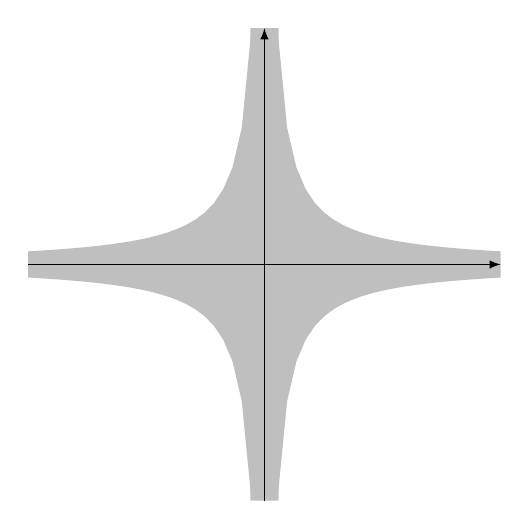
\begin{tikzpicture}
    	\fill [lightgray, domain=-3:-0.17, variable=\x]
      	(-3, 0)
      	-- plot ({\x}, {0.5*1/\x})
      	-- (-0.17, 0)
      	-- cycle;
    	\fill [lightgray, domain= -3: -0.17, variable=\x]
      	(-3, 0)
      	-- plot ({\x}, {-0.5*1/\x})
      	-- (-0.17, 0)
      	-- cycle;
    	\fill [lightgray, domain=0.17:3, variable=\x]
      	(0.17, 0)
      	-- plot ({\x}, {0.5*1/\x})
      	-- (3, 0)
      	-- cycle;
    	\fill [lightgray, domain=0.17:3, variable=\x]
      	(0.17, 0)
      	-- plot ({\x}, {-0.5*1/\x})
      	-- (3, 0)
      	-- cycle;	
    	\fill [lightgray, domain= -0.18:0.18, variable=\x]
      	(-0.18, 3)
      	-- plot ({\x}, {0})
      	-- (0.18 , 3)
      	-- cycle;
    	\fill [lightgray, domain= -0.18:0.18, variable=\x]
      	(-0.18, -3)
      	-- plot ({\x}, {0})
      	-- (0.18 , -3)
      	-- cycle;

    		\coordinate (XAxisMin) at (-3,0);
    		\coordinate (XAxisMax) at (3,0);
    		\coordinate (YAxisMin) at (0,-3);
    		\coordinate (YAxisMax) at (0,3);
    		\draw [thin,-latex] (XAxisMin) -- (XAxisMax);% Draw x axis
    		\draw [thin,-latex] (YAxisMin) -- (YAxisMax);% Draw y axis	
	\end{tikzpicture}  

	\caption{The region $X_t=\{(x,y) \in \R^2 \colon |xy| \leq t\}$. \label{fig:fundex}}
	\end{figure}
\end{rem}


\begin{cor}\label{cor:finite}
Every class in $\Cl_K$ contains an integral ideal of norm at most $ \left(\dfrac{\pi}{4}\right)^s \dfrac{n!}{n^n} |\disc K|^{1/2}$. In particular, $\Cl_K$ is finite. 
\end{cor}

\pf Take $\kappa \in \Cl_K$. Choose an integral ideal $I$ such that $[I]= \kappa^{-1}$. By Theorem~\ref{thm:finite}, there is a nonzero $\alpha \in I$ with
	\[
	|\Nm{K/\Q}(\alpha)| \leq M_K N(I).
	\]
Let $J=\alpha I^{-1} \subseteq \O_K$. By construction, $[J]=[I^{-1}]=[I]^{-1}=\kappa$ as these classes are equal up to a prime ideal. However,
	\[
	N(J)N(I)= N(JI)= N(\alpha \O_K)= |\Nm{K/\Q}(\alpha)| \leq M_K N(I),
	\]
so that $N(J) \leq M_K$. Therefore as there are only finitely many ideals of $\O_K$ with a given norm, $\Cl_K$ is finite. \qed \\

\begin{cor}\label{cor:generated}
$\Cl_K$ is generated by equivalence classes of prime ideals with norm at most $\left(\dfrac{\pi}{4}\right)^s \dfrac{n!}{n} |\disc K|^{1/2}$. 
\end{cor}

\pf \emph{(Sketch)} Write $I= \p_1^{e_1} \cdots \p_r^{e_r}$. Then $[I]=[\p_1]^{e_1} \cdots [\p_r]^{e_r}$ in $\Cl_K$. However, $N(I)=N(\p_1)^{e_1} \cdots N(\p_r)^{e_r}$. The result then follows from Corollary~\ref{cor:finite}. \qed \\



\subsection{Discriminant Bounds}

Now given a fixed discriminant $D$, how many number fields $K$ are there such that $\disc K=D$? It turns out $\#\{ K/\Q \colon [K \colon \Q]<\infty, \disc K=d\}$ is finite. 

\begin{prop}
For any integer $d$, there are only finitely many $n \geq 1$ for which there is a number field $K/\Q$ of degree $n$ and discriminant $d$. 
\end{prop}

By Corollary~\ref{cor:finite}, every class of $\Cl_K$ contains an integral ideal of norm at most $M_K:=\left(\frac{\pi}{4}\right)^s \frac{n!}{n^n} |\disc K|^{1/2}$. Since the norm of an ideal is at least 1, we have a lower bound for $M_K$:
	\[
	1 \leq \left(\dfrac{\pi}{4}\right)^s \dfrac{n!}{n^n} |\disc K|^{1/2}=: M_K
	\]
But then for $\disc K$, we have
	\[
	\sqrt{|\disc K|} \geq \left(\dfrac{\pi}{4}\right)^s \dfrac{n^n}{n!}.
	\]
We can obtain a slightly weaker inequality by using $\frac{\pi}{4}<1$ and $s \leq \frac{n}{2}$. Then we have
	\[
	|\disc K|^{1/2} \geq \left(\dfrac{\pi}{4}\right)^{n/2} \dfrac{n^n}{n!}.
	\]
If $a_n= \left(\frac{\pi}{4}\right)^{n/2} \frac{n^n}{n!}$, then 
	\[
	\dfrac{a_{n+1}}{a_n}= \left(\dfrac{\pi}{4}\right)^{1/2} \left(1+ \dfrac{1}{n}\right)^n \ma{n \to \infty} e\sqrt{\dfrac{\pi}{4}}
	\] \qed \\


If $K \neq \Q$, i.e. $[K \colon \Q]>1$, then we have
	\[
	\sqrt{|\disc K|} \geq \left(\dfrac{\pi}{4}\right)^{2/2} \dfrac{2^2}{2!}= \dfrac{\pi}{2}>1.
	\]
Hermit then used this fact to show the following:

\begin{thm}[Hermite] \label{thm:hermite}
For any number field $K \neq \Q$, $\disc K \neq \pm 1$. In particular, there is a prime $p$ that ramifies in $K$. 
\end{thm}


As an interesting application of this, which is otherwise difficult to prove, we have the following:

\begin{prop}
Let $K,L$ be number fields such that $\gcd(\disc K, \disc L)=1$. Then $K \cap L=\Q$. 
\end{prop}

\pf Define $E:= K \cap L$ and suppose that $p$ ramifies in $E$. Then $p$ must ramify in both $K$ and $L$. The ramification degree of $\p$ over $p$ must be greater than 1 so that
	\[
	e(\P/\p)= e(\P/\p)e(\p/p)>1.
	\]
Now $\P$ ramifies in $K$ so that $p \mid \disc K$. Similarly, $p \mid \disc L$. But then $\gcd(\disc K, \disc L)>1$, a contradiction. Therefore, no prime ramifies in $E$. By Theorem~\ref{thm:hermite}, it must be that $E=\Q$. \qed \\

One can use this idea to prove interesting results for the composite of fields. 

\begin{prop}
Let $K,L$ be number fields such that $\gcd(\disc K, \disc L)=1$. Then if $F=KL$,
\begin{enumerate}[(i)]
\item $\O_F= \O_K\O_L$
\item if $\{x_i\}$ is an integral basis of $K$ and $\{y_j\}$ is an integral basis for $L$, then $\{x_i y_j\}$ is a basis for $F$
\item $\disc F= (\disc K)^{[L \colon \Q]} (\disc L)^{[K \colon \Q]}$
\end{enumerate}
\end{prop}


\begin{thm}
For $d \in \Z$, there are only finitely many number fields, up to isomorphism, with discriminant $d$.
\end{thm}

\pf It suffices to consider number fields $K$ with a fixed degree $n$ as
	\[
	|\disc K|^{1/2} \geq \left(\dfrac{\pi}{4}\right)^s \dfrac{n^n}{n!} \geq \left(\dfrac{\pi}{4}\right)^{n/2} \dfrac{n^n}{n!}
	\]
so that for sufficiently large $n$, the inequality fails. Fix a number field $K$ of degree $n>1$ (the case where $n=1$ is trivial) and let $d=\disc K$. Consider $\iota: \O_K \hookrightarrow \R^n$. Let $\sigma_1,\ldots,\sigma_r: K \hookrightarrow \R$ be the $r$ real embeddings of $K$ into $\R$ and let $\sigma_{r+1},\ldots,\sigma_{r+s}, \overline{\sigma_{r+1}}, \ldots, \overline{\sigma_{r+s}}: K \hra \C$ be the $2s$ complex embeddings of $K$ into $\C$. The map $\iota: \O_K \to \R^n$ can be given by
	\[
	\iota(\alpha)= \big(\sigma_1(\alpha),\ldots,\sigma_r(\alpha), \imag(\sigma_{r+1}(\alpha)), \ldots, \imag(\sigma_{r+s}(\alpha)), \ream(\sigma_{r+1}(\alpha)), \ldots, \ream(\sigma_{r+s}(\alpha)) \big).
	\]
Fix a constant $C>0$ and define 
	\[
	X:= \{ x \in \R^n \colon |x_1| \leq C, |x_i| \leq \frac{1}{2} \text{ for } i\geq 2\}.
	\]
Because $X$ is a hypercube, it is clear that $X$ is compact, symmetric, and convex. For some constant $r_n$, depending on $n$, we have $\vol X \gg r_nC$. Take $C$ sufficiently large (recalling this depends on $n$ and $d$) so that $\vol X \geq 2^n \covol(\iota(\O_K))= 2^n |\disc K|^{1/2}=2^n \sqrt{|d|}$. 

Minkowski's Theorem (Theorem~\ref{thm:mink}) says there exists a nonzero $\alpha \in \O_K$ such that $\iota(\alpha) \in X$. For real $\sigma_i$, $|\sigma_i(\alpha)| \leq \frac{1}{2}<1$ while for complex $\sigma_i$, $|\sigma_i(\alpha)| \leq \sqrt{(1/2)^2+(1/2)^2}<1$. Therefore, $|\sigma_i(\alpha)|<1$ for $i \geq 2$. But then $|\sigma_1(\alpha)|>1$ since 
	\[
	1 \leq |\Nm{K/\Q}(\alpha)|= \prod_{\sigma: K \hra \C} |\sigma(\alpha)|.
	\]
and $\Nm{K/\Q}(\alpha) \in \Z$ so that all $|\sigma(\alpha)|$ cannot be less than 1. 


We claim that $K=\Q(\alpha)$: if $p_\alpha$ is the minimal polynomial of $\alpha$, then
	\[
	\prod_{\sigma: K \hra \C} \big( x-\sigma(\alpha) \big)= p_\alpha(x)^{[K \colon \Q(\alpha)]}.
	\]
We show that $\sigma_1(\alpha) \neq \sigma(\alpha)$ for $\sigma \neq \sigma_1$. This will show that $\sigma_1(\alpha)$ is a root of multiplicity 1, forcing the exponent to be 1. This will show that $[K \colon \Q(\alpha)]=1$, forcing $K=\Q(\alpha)$. For $\sigma \notin \{\sigma_1, \overline{\sigma_1}\}$, $|\sigma(\alpha)|<1$. But then $\sigma(\alpha) \neq \sigma_1(\alpha)$ as $|\sigma_1(\alpha)|>1$. Furthermore, $\sigma_1(\alpha) \neq \overline{\sigma_1(\alpha)}$ as $|\ream(\sigma_1(\alpha))|<\frac{1}{2}$. But then $\imag(\sigma_1(\alpha)) \neq 0$ as $|\sigma_1(\alpha)|>1$. 

Now $|\sigma(\alpha)|$ is bounded by some constant (depending only on $n$ and $d$ for all $\sigma: K \hra \C$). Therefore, the coefficients of $p_\alpha$ are bounded in terms of $n$ and $d$. Then there are finitely many possible $p_\alpha$ since $p_\alpha \in \Z[x]$. Then there are only finitely many $K=\Q(\alpha)$, up to isomorphism. \qed \\

\begin{ex}
For number fields to be isomorphic, it is necessary that they have the same discriminant. However, this is not sufficient. There are non-isomorphic fields with the same discriminant: Let $\alpha$ be a root of $p_\alpha(x)=x^4-6$ and $\beta$ be a root of $p_\beta(x)=x^4-24$. Define $K=\Q(\alpha)$ and $L=\Q(\beta)$. We have $\disc K=\disc L = -2^{11} \cdot 3^3$. To tell that the fields are distinct, we examine how primes factor in $K$ and in $L$. In $\O_K$, $5\O_K= \p_1\p_2\p_3\p_4$ while in $\O_L$, $5\O_L=\q_1\q_2$. Therefore, $K$ and $L$ are not isomorphic. \xqed
\end{ex}



